% $Id: introduction.tex 34630 2013-04-29 22:53:51Z roldeman $

\section{The \boldmath $\alpha_T$ analysis at CMS}
\label{sec:Introduction}

%%%%%%% MY BIT

The Standard Model (SM) of particle physics \cite{Salam1964}\cite{Glashow1961}\cite{Weinberg1967} has consistently stood up to experimental scrutiny. Despite its successes in describing fundamental particles and their interactions, there are experimental and theoretical inconsistencies that imply the SM is incomplete. One favoured extension of the SM is supersymmetry (SUSY), predicting the existence of a new particle for every SM particle. Whilst being theoretically well motivated, SUSY at the TeV scale can act to solve the Higgs hierarchy problem and provide a candidate dark matter particle \cite{SUSYprimerMartin:1997ns}\cite{more(See alphaT papter)}.
\\\\
% the LHC and cms
The Large Hadron Collider (LHC) \cite{LHCMachine} is in the final stages of preparation for Run 2, in which the centre of mass of the proton collisions will increase from the $8$~TeV in Run 1 to $13$~TeV. The CMS detector is built around one of the proton collision points. It is a multi-purpose, hermetic particle detector designed to be sensitive to the production of unobserved particles. The CMS detector contains a $~4$~Tesla magnet that bends charged particles to allow accurate determination of their momenta. These particles pass through the silicon tracking system, electromagnetic and hadronic calorimeters and finally the muon chambers. From the traces left behind in each of these subdetectors, the type of particle produced in the collision can be identified. The momentum of charged particles can be measured with a resolution of greater than $99\%$ \cite{ScienceArticle} \cite{CMSTechDesign1DetectorPerformance}. For a detailed description of the CMS detector see \cite{CMS_Overview_Chatrchyan:2008aa}.
\\\\
As the LHC is a proton collider, the highest cross section SUSY production processes occur via strong force interactions. In the case of R parity conserving SUSY, this results in the pair production of gluinos or squarks that rapidly decay to a weakly interacting Lightest Supersymmetric Particle (LSP) \cite{SUSYPhe_hadronic_states_Farrar:1978xj}. The typical signature left in the CMS detector is one of hard hadronic jets with significant missing momentum carried away by the undetected LSP. The $\alpha_T$ analysis is designed to minimise the SM background while searching for SUSY produced in this purely hadronic way. As the exact momentum along the beam direction of the colliding partons is not known, the momentum and missing momentum of particles is only considered transverse to the beam direction.

\subsection{Definition of \boldmath $\alpha_T$}

Due to the very high cross sections of QCD processes at the LHC, there is a large multijet background. In the case that one of the jets are mismeasured, this results in fake missing energy, the signature left by SUSY production. To negate this effect, the dimensionless variable $\alpha_T$ is introduced \cite{AlphaTproposalCMS:2008vya} \cite{AlphaTproposalPhysRevLett.101.221803}. For a dijet system it is defined as:
\begin{equation}
\alpha_T=\frac{E_T^{j_2}}{M_T},
\end{equation}
where $E_T^{j_2}$ is the energy of the lowest energy jet, $M_T=\sqrt{H_T^2-\cancel{H}_T^2}$ is the invariant mass of the dijet system. It is constructed from the jet characterising variables:
\begin{equation}
H_T=\sum_{i=1}^{n_{jet}}E_T^{j_i}, 
\end{equation}
and
\begin{equation}
\cancel{H}_T=|\sum_{i=1}^{n_{jet}}\vec{p}_T^{j_i}|,
\end{equation}
with $n_{jet}$ jets, $j_i$, with transverse momentum $\vec{p}_T^{j_i}$ and transverse energy $E_T^{j_i}$. For events with more than two jets, a pseudo dijet system is formed by combining jets. The system chosen is one that minimises $|\Delta H_T|$, this is the difference between the $E_T$ of each pseudo jet, where $E_T$ is the scalar sum of the transverse energies of all the jets in each pseudo jet. This leads to a generalised form of $\alpha_T$ \cite{AlphaT8TeVChatrchyan:2013lya}:
\begin{equation}
\alpha_T=\frac{1}{2}\times\frac{H_T-\Delta H_T}{\sqrt{H_T^2-\cancel{H}_T^2}}
\end{equation}
Balanced and mismeasured multijet events have values of $\alpha_T\leq0.5$, while events with genuine missing energy have values of $\alpha_T>0.5$. By choosing an appropriate cut above $0.5$ it is possible to reduce the multijet background to a negligible amount, this is evident in Fig.~\ref{fig:alphaT}. 

\begin{figure}
	\begin{center}
		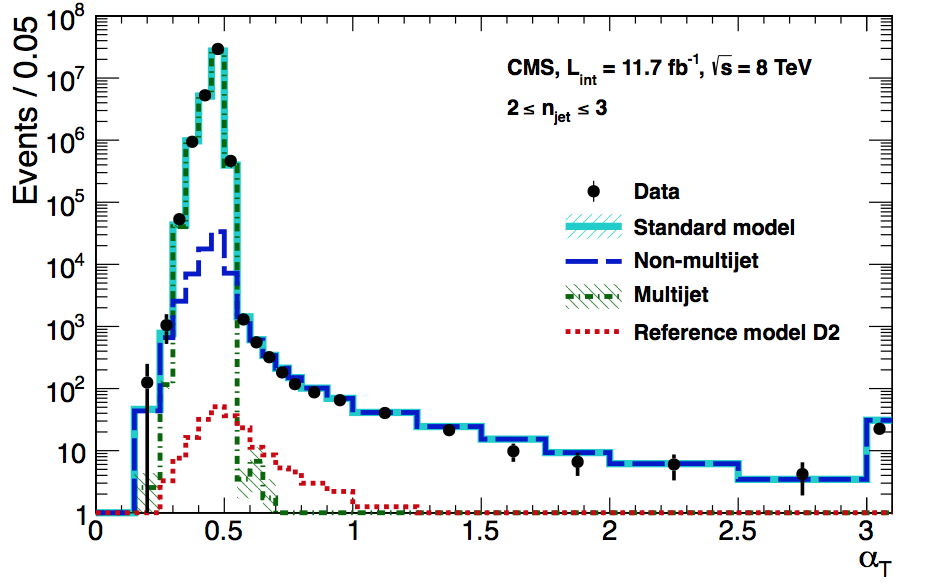
\includegraphics[width=0.8\linewidth]{alphaT1_bkgd}
	\end{center}
	\caption{The $\alpha_T$ values for events with $H_T>375$ GeV and 2 to 3 jets that pass all other cuts imposed in the $\alpha_T$ analysis. The green dotted line shows the expected multijet QCD background that can be removed with an appropriate cut on $\alpha_T$ \cite{AlphaT8TeVChatrchyan:2013lya}}
	\label{fig:alphaT}
\end{figure}

\subsection{The \boldmath $\alpha_T$ analysis}

The only genuine source of missing transverse energy ($\cancel{E}_T$) in the SM is electroweak neutrino production. In these cases an associated lepton is simultaneously produced. This background is minimised by vetoing any events with isolated \footnote{A particle is isolated if the energy of other particles within a cone of $R\equiv\sqrt{(\Delta\phi)^2+(\Delta\eta)^2}=0.3$, where $\phi$ is the azimuthal angle and $\eta$ the pseudorapidity, do not add up to a significant proportion of the particle's momentum, typically $~10$\%} leptons of $p_T>10$~GeV. To ensure a fully hadronic final state there is also a veto on photons of $p_T>25$~GeV. Further, to reduce the ``lost leptons'' backgrounds from W~+~jets 
and $t\bar{t}$, events containing single isolated tracks with $p_T >10$~GeV and $|\eta| < 2.5$ are vetoed.
\\\\
Events are also required to contain at least one $p_T>100$~GeV and one $p_T>40$~GeV jets, where the jets are well reconstructed in the central region, $|\eta|<3$. If any jets fall outside the $\eta$ range, the event is vetoed. Significant hadronic activity is selected for by requiring $H_T>200$~GeV. Events are categorised based on the number of jets, the number of jets with a reconstructed b-quark and the value of $H_T$. 
\\\\
Due to the reduction in QCD cross section at high values of $H_T$ the $\alpha_T$ cut is reduced with this variable while keeping a consistent effective $\cancel{H_T}$ value, see Table~\ref{tab:alphat-thresholds}. Additional cleaning cuts on the ratio of $\cancel{H_T}/\cancel{E_T}$ are also required to reduce instances of high $\cancel{H_T}$ caused by jets just falling out of acceptance. Full details of the analysis as carried out on Run~1 data can be found at \cite{AlphaT8TeVChatrchyan:2013lya} and \cite{AlphaT_7TeV_PRLChatrchyan:2011zy}, and ongoing developments for Run~2 at \cite{AN-15-004}.
\\\\

\begin{table}[h!]
  \caption{$\alpha_T$ and (effective) $\cancel{H_T}$ thresholds per $H_T$ bin.\label{tab:alphat-thresholds}}
  \centering
  \footnotesize
  \begin{tabular}{ lcccccc }
    \hline
    \hline
    $H_T$     & 200--250   & 250--300   & 300--350  & 350--400  & 400--800 \\ %& $>$900       \\
    \hline                                                                     
    $alpha_T$      & 0.65       & 0.60       & 0.55      & 0.53      & 0.52     \\  %& 0.505         \\
    "Min $\cancel{H_T}$"   & $\sim$128  & $\sim$138  & $\sim$125 & $\sim$133 & $\sim$137 \\  %& $\sim$126 \\
    \hline
    \hline
  \end{tabular}
\end{table}

\noindent For the prediction of backgrounds and measuring of systematic errors, control samples are defined. These have all the cuts used for the signal selection described above, but require the existence of one or two leptons or a photon. These leptons and photons are ignored in the calculation of any analysis variables. Additionally, in the case of the lepton control sample no, $\alpha_T$ requirement is made.